\documentclass[letterpaper,12pt,leqno]{article}
\usepackage{paper}
\bibliographystyle{bibliography}

% Enter paper title:
\hypersetup{pdftitle={Paper Example}}

% Enter permanent URL to paper
%\available{https://github.com/pmichaillat/latex-paper}

% Enter BibTeX file with references:
\newcommand{\bib}{bibliography.bib}

% Enter PDF file with figures here:
\newcommand{\pdf}{figures.pdf}

% Fill out paper:
\begin{document}
\title{Rural Accessibility in Indonesia: Fuel Subsidy versus Infrastructure Development}
\author{Maghfira Ramadhani
\thanks{Maghfira Ramadhani: Georgia Institute of Technology. Acknowledgements.}}
\date{March 2023}                       
\begin{titlepage}\maketitle

Indonesia have been subsidizing transportation cost for a long time.

\end{titlepage}\section{Introduction}\label{s:introduction}
 
\paragraph{Research question} Lorem ipsum dolor sit amet,  pariatur.\footnote{Excepteur sint, sunt in culpa qui officia deserunt mollit anim id est laborum.}

\paragraph{Answer to the question} Lorem ipsum dolor sit amet. Duis aute irure dolor in reprehenderit in voluptate velit esse cillum dolore eu fugiat nulla pariatur. 

\paragraph{Related literature} This study build insight from previous research regarding impact evaluation of government programs on village-level development. \citet{asher_2020} .\footnote{In reprehenderit in eu fugiat nulla pariatur \citep{LMS18a}.}


\paragraph{Outline} The rest of the paper is organized as follows. I develop the conceptual framework for the discussion in Section \ref{s:framework}. Section \ref{s:context} describe the institutional context and background of infrastructure development agenda in Indonesia. I provide the data and the descriptive statistics along with preliminary evidence in Section \ref{s:strategy}. Section \ref{s:conclusion} provides a concluding remark of the discussion.

\section{Conceptual Framework}\label{s:framework}

In this section, I discussed the conceptual framework for understanding the impact of ... on rural accesibility.

\subsection{Accessibility in rural area}

Connectivity challenges in Indonesia \citep{sandee_2016}. Regarding rural accessibility, the challenge mainly related to intra-island connectivity ---links within individual islands--- is linking underdeveloped regions to growth centers. In the densely populated part of Java island, the city as the center of growth, the challenges of connectivity is mostly congestion-based challenge causing high-cost for mobility. In contrast, in the rural areas of Java, we can still find a village that we can only access by motorcycle or even only by foot. This challenge is somewhat similar in other main islands such as Sumatra, Kalimantan, Sulawesi and Papua. In these other mainlands, the challenges are the existence of adequate and reliable infrastructure that drives up the transportation cost.

\subsection{Transportation demand in rural area} 

\begin{proposition}\label{p:type1}  Lorem ipsum dolor sit amet $z \in \mathbb{R}$, consectetur adipiscing elit
\begin{equation}
\bm{S}^*(z) = \frac{S(z)}{23 -\zeta\gamma [45- S(z)] + \ln(y)}.
\label{e:type1}\end{equation}
Ut enim ad minim veniam, sunt in culpa qui officia deserunt mollit anim id est laborum:
\begin{equation}
\mathcal{S}^*(z) = S(z) \times \mathbb{E}(N(z)) + \alpha \beta - \sum_{i=0}^{+\infty}\mathcal{F}^{i}-\exp(\lambda \mu).
\label{e:type1steps}\end{equation}
\end{proposition}

\begin{proof} There is a simple proof to this result. It gives equation \eqref{e:type1steps}.\end{proof} 

Quis autem vel eum iure reprehenderit, qui in ea voluptate velit esse, quam nihil molestiae consequatur $\bm{\alpha(X)}$. Duis aute irure dolor in reprehenderit in voluptate velit esse cillum \eqref{e:type1}, excepteur sint occaecat cupidatat non proident $z^*$:
\begin{equation*}
\frac{\mathcal{S}(z^*)}{1 -\theta + \theta \mathcal{S}(z^*)} = \sum_{i=0}^{+\infty}F^{i} - \Lambda(i).
\end{equation*}
From this definition we obtain the following results (details of the proof are relegated to appendix~\ref{a:appendix1}):

\begin{lemma}\label{p:cv} Ut enim ad minim veniam, quis nostrud exercitation ullamco laboris nisi ut aliquip ex ea commodo consequat $\alpha$:
\begin{equation}
z^* = \int_{0}^{\infty} \alpha(i) \cdot \frac{1-\beta}{1-\alpha(i)\beta}\,di.
\label{e:cv}\end{equation}
Consectetur adipiscing elit, sed do eiusmod tempor incididunt ut labore et dolore magna aliqua $\mathcal{Z}(\alpha)$. \end{lemma}

Ut enim ad minima veniam, quis nostrum exercitationem ullam corporis suscipit laboriosam, nisi ut aliquid ex ea commodi consequatur? Combining equation \eqref{e:cv} with other results, we obtain the following corollary (the proof is in appendix~\ref{a:subappendix}): 

\begin{corollary} Lorem ipsum dolor sit amet, consectetur adipiscing elit, sed do eiusmod tempor incididunt ut labore et dolore magna aliqua:
\begin{equation*}
\mathbb{E}(N(z^*)) \approx \frac{1-\mathbb{P}(\alpha\pi)}{1-\pi}- \frac{f(y)}{z(p)^*} +P(\Gamma).
\end{equation*}\end{corollary}

\subsection{Component of Transport Cost}

Indonesia have been subsidizing fuel subsidy for a long time. It is argued that subzidizing fuel will bring development.

\section{Institutional Context and Background}\label{s:context}

The government initiatives in attracting foreign capital and facilitating public-private partnership in bringing a large-scale infrastructure development has been a policy priority since 2015 \citep{pwc_2016}.

\subsection{Fossil Fuel Subsidy Regime}

Indonesia used to be a large oil exporter in the oil boom period in 1970s and 1980s and the National Oil Company (NOC), Pertamina contributed a big part in delivering the subsidy to the public. 

\subsection{Decentralization of Development}

Figure~\ref{f:graph1} depicts the result.


\begin{figure}[t]
\subcaptionbox{Village status in 2014\label{f:panel1}}{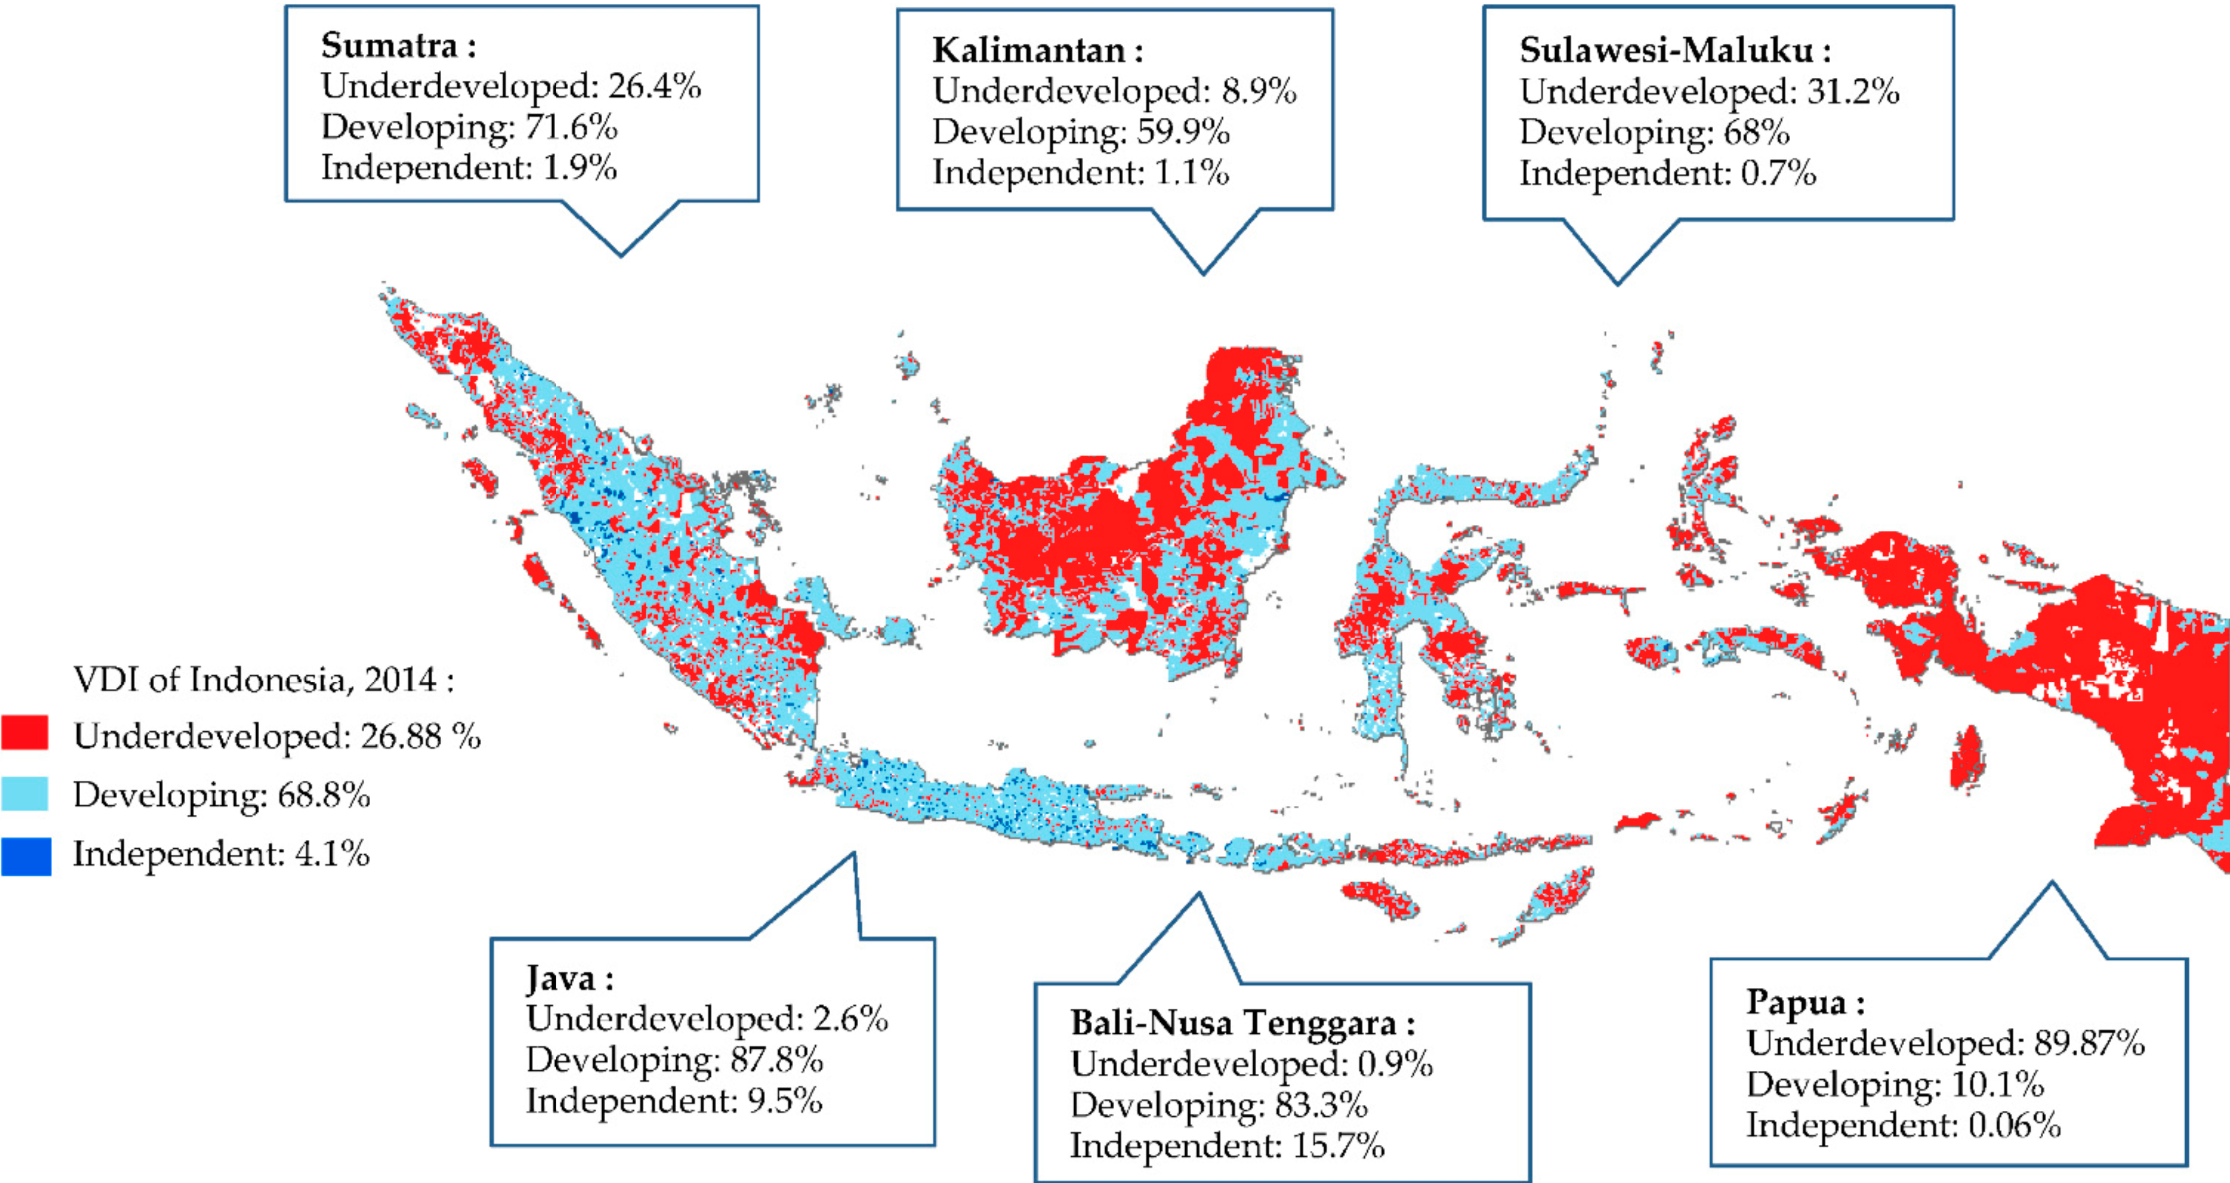
\includegraphics[scale=0.2]{Final_Project/image/vdi2014.png}}\hfill
\subcaptionbox{Village status in 2018\label{f:panel2}}{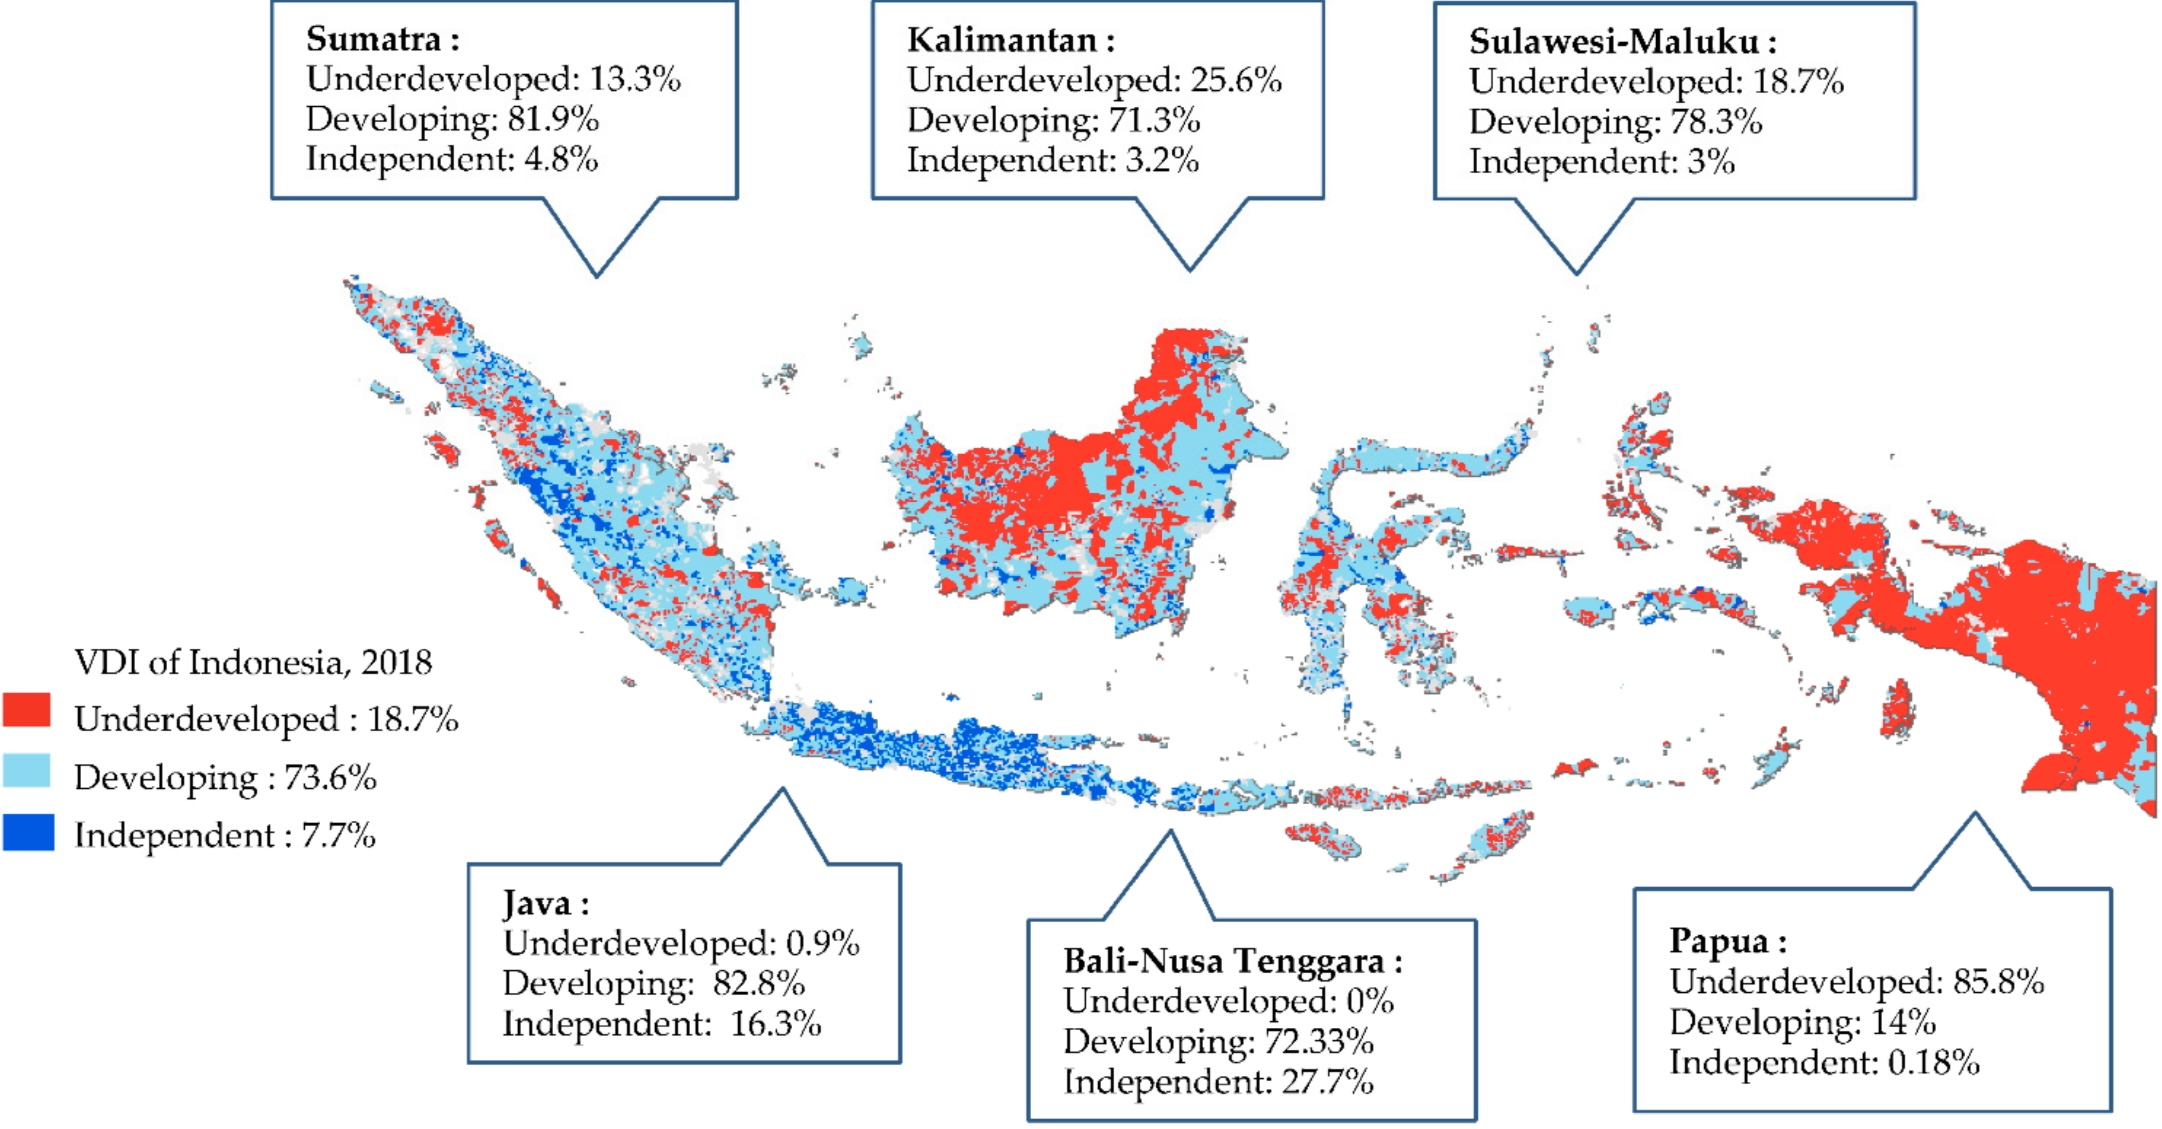
\includegraphics[scale=0.205]{Final_Project/image/vdi2018.jpg}}
\caption{Indonesia's VDI's status}
\note{Source: Statistics Indonesia \citet{hartojo_2022}}
\label{f:graph1}\end{figure}

\section{Empirical Strategy}\label{s:strategy}

I observed village level as the unit of analysis. I obtained a proprietary Village Potential Statistics data for the year 2011, 2014 and 2018 from Indonesia's Central Bureau of Statistics consisting of consecutively 77,961, 82,190, and 83,931 observations of village in rural and urban areas. The original survey covers the general information of village, population and employment, housing and environment, natural disaster, education and health, sport and leisure, transportation and communication, land use, economic activity, security, local government, community empowerment, and agriculture. However, the data on transportation cost are not collected in the year 2011, and also the data about village government budget is not available for the year 2018. 

\subsection{Data and Descriptive Statistics}

At vero eos et accusamus et iusto odio dignissimos ducimus, qui blanditiis praesentium voluptatum deleniti atque corrupti, quos dolores et quas molestias excepturi sint, obcaecati cupiditate non provident, similique sunt in culpa, qui officia deserunt mollitia animi, id est laborum et dolorum fuga. 

\paragraph{Paragraph title} Et harum quidem rerum facilis est et expedita distinctio. Nam libero tempore, cum soluta nobis est eligendi optio, cumque nihil impedit, quo minus id, quod maxime placeat, facere possimus, omnis voluptas assumenda est, omnis dolor repellendus. Temporibus autem quibusdam et aut officiis debitis aut rerum necessitatibus saepe eveniet, ut et voluptates repudiandae sint et molestiae non recusandae. 

\subsection{Measuring Rural Accessibility with Transport Cost}

\paragraph{Another paragraph} Itaque earum rerum hic tenetur a sapiente delectus, ut aut reiciendis voluptatibus maiores alias consequatur aut perferendis doloribus asperiores repellat. Nam libero tempore, cum soluta nobis est eligendi optio, cumque nihil impedit, quo minus id, quod maxime placeat, facere possimus, omnis voluptas assumenda est, omnis dolor repellendus. 

\paragraph{Another result in a panel} Nam libero tempore, cum soluta nobis est eligendi optio, cumque nihil impedit, quo minus id, quod maxime placeat, facere possimus, omnis voluptas assumenda est, omnis dolor repellendus. Figure \ref{f:panel1} displays cum soluta nobis est eligendi optio, cumque nihil impedit. Quod maxime placeat, facere possimus, omnis voluptas assumenda est in figure \ref{f:panel2}.

\subsection{Preliminary Findings}

A full-page graph is on figure \ref{f:graph2}. Nam libero tempore, cum soluta nobis est eligendi optio, cumque nihil impedit, quo minus id, quod maxime placeat, facere possimus, omnis voluptas assumenda est, omnis dolor repellendus.

\begin{figure}[p]
\subcaptionbox{Caption for panel}{\includegraphics[scale=\sfig,page=1]{\pdf}}\hfill
\subcaptionbox{Caption for panel}{\includegraphics[scale=\sfig,page=2]{\pdf}}\vfig
\subcaptionbox{Caption for panel}{\includegraphics[scale=\sfig,page=3]{\pdf}}\hfill
\subcaptionbox{Caption for panel}{\includegraphics[scale=\sfig,page=4]{\pdf}}\vfig
\subcaptionbox{Caption for panel}{\includegraphics[scale=\sfig,page=5]{\pdf}}\hfill
\subcaptionbox{Caption for panel}{\includegraphics[scale=\sfig,page=1]{\pdf}}
\caption{Caption for the graph}
\note{Note for the graph. Nam libero tempore, cum soluta nobis est eligendi optio, cumque nihil impedit, quo minus id, quod maxime placeat from \citet[section 3]{MS22b}.}
\label{f:graph2}\end{figure}


\paragraph{Another paragraph} At vero eos et accusamus et iusto odio dignissimos ducimus, qui blanditiis praesentium voluptatum deleniti atque corrupti, quos dolores et quas molestias excepturi sint, obcaecati cupiditate non provident, similique sunt in culpa, qui officia deserunt mollitia animi, id est laborum et dolorum fuga. Et harum quidem rerum facilis est et expedita distinctio. Nam libero tempore, cum soluta nobis est eligendi optio, cumque nihil impedit, quo minus id, quod maxime placeat, facere possimus, omnis voluptas assumenda est, omnis dolor repellendus. Temporibus autem quibusdam et aut officiis debitis aut rerum necessitatibus saepe eveniet, ut et voluptates repudiandae sint et molestiae non recusandae. Itaque earum rerum hic tenetur a sapiente delectus, ut aut reiciendis voluptatibus maiores alias consequatur aut perferendis doloribus asperiores repellat. 

\paragraph{Yet another paragraph} At vero eos et accusamus et iusto odio dignissimos ducimus, qui blanditiis praesentium voluptatum deleniti atque corrupti, quos dolores et quas molestias excepturi sint, obcaecati cupiditate non provident, similique sunt in culpa, qui officia deserunt mollitia animi, id est laborum et dolorum fuga. Et harum quidem rerum facilis est et expedita distinctio. Nam libero tempore, cum soluta nobis est eligendi optio, cumque nihil impedit, quo minus id, quod maxime placeat, facere possimus, omnis voluptas assumenda est, omnis dolor repellendus. Temporibus autem quibusdam et aut officiis debitis aut rerum necessitatibus saepe eveniet, ut et voluptates repudiandae sint et molestiae non recusandae. Itaque earum rerum hic tenetur a sapiente delectus, ut aut reiciendis voluptatibus maiores alias consequatur aut perferendis doloribus asperiores repellat. 


\begin{table}[t]
\caption{Caption for the table}
\begin{tabular*}{\textwidth}[]{p{3.3cm}@{\extracolsep\fill}cccc}
\toprule
& Timeline & Natural rate & Monetary  & Government \\
&  & of interest &  policy & spending\\
\midrule
\multicolumn{5}{l}{A. Qui dolorem eum fugiat}\\
ZLB: & $t\in (0,T) $ & $r^n<0$ & $i=0$  & -- \\
Normal times: & $t>T$ &  $r^n>0$ & $i= r^n + \phi \pi$  & --   \\
\midrule
\multicolumn{5}{l}{B. Nam libero tempore, cum soluta nobis}\\
ZLB: & $t\in (0,T)$ & $r^n<0$ & $i=0$  & -- \\
Forward guidance: & $t\in (T,T+\Delta)$ & $r^n>0$ & $i=0$  & --\\
Normal times: & $t>T+\Delta$ & $r^n>0$ & $i= r^n + \phi \pi$  & -- \\
\midrule
\multicolumn{5}{l}{C. At vero eos et accusamus}\\
ZLB: & $t\in (0,T) $ & $r^n<0$ & $i=0$  & $g>0$  \\
Normal times: & $t>T$ & $r^n>0$ & $i= r^n + \phi \pi$  & $g=0$   \\
\bottomrule
\end{tabular*}
\note{Temporibus autem quibusdam et aut officiis debitis aut rerum necessitatibus saepe eveniet, ut et voluptates repudiandae sint et molestiae non recusandae. Ut aut reiciendis voluptatibus maiores alias consequatur aut perferendis doloribus asperiores repellat \citep[table 1]{MS21a}.}
\label{t:table}\end{table}

\section{Conclusion}\label{s:conclusion}

To conclude, at vero eos et accusamus et iusto odio dignissimos ducimus, qui blanditiis praesentium voluptatum deleniti atque corrupti, quos dolores et quas molestias excepturi sint, obcaecati cupiditate non provident, similique sunt in culpa, qui officia deserunt mollitia animi, id est laborum et dolorum fuga. 

At vero eos et accusamus et iusto odio dignissimos ducimus, qui blanditiis praesentium voluptatum deleniti atque corrupti, quos dolores et quas molestias excepturi sint.

\bibliography{\bib}

% Fill out appendix:
\newpage
\appendix
\section{Appendix title}\label{a:appendix1}

We extend the model of section~\ref{s:section} by introducing a quadratic cost. Obcaecati cupiditate non provident, similique sunt in culpa, qui officia deserunt mollitia animi, id est laborum et dolorum fuga. 

\subsection{Subsection title} 

At vero eos et accusamus et iusto odio dignissimos ducimus, qui blanditiis praesentium voluptatum deleniti atque corrupti, quos dolores et quas molestias excepturi sint, obcaecati cupiditate non provident, similique sunt in culpa, qui officia deserunt mollitia animi, id est laborum et dolorum fuga. 

\subsection{Another subsection}

 Et harum quidem rerum facilis est et expedita distinctio. Nam libero tempore, cum soluta nobis est eligendi optio cumque nihil impedit quo minus id quod maxime placeat facere possimus, omnis voluptas assumenda est, omnis dolor repellendus \citep{MS22a}. A corrolary in the appendix is as follows:

\begin{corollary} Similique sunt in culpa, qui officia deserunt mollitia animi, id est laborum et dolorum fuga:
\begin{equation*}
\mathbb{E}(\Omega) = \mathbb{P}(\omega\cdot \mu - \xi) - \sum_{i=0}^{m}\sum_{j=-\infty}^{n} \sigma(i,j) + 123^{56}.
\end{equation*}\end{corollary}

\paragraph{A paragraph with some math} Temporibus autem quibusdam $\xi$ et aut officiis debitis aut rerum necessitatibus saepe eveniet ut et voluptates repudiandae sint et molestiae non recusandae $1-\gamma$. Itaque earum rerum hic $S(z^*)$ tenetur a sapiente delectus $\mathcal{B}^\theta$, ut aut reiciendis voluptatibus maiores alias consequatur aut perferendis doloribus asperiores repellat $\mathcal{V}^i$. Aggregating these scenarios, we obtain the continuation value:
\begin{equation}
\mathbb{V}^r = (1-\gamma) \times 0 +\gamma S(z^*) v^s+\gamma [1-S(z^*)] \mathcal{V}^i-c.
\label{e:appendix1}\end{equation}

\paragraph{Paragraph with links to appendix equations} Ut enim ad minima veniam, quis nostrum exercitationem ullam corporis suscipit laboriosam, nisi ut aliquid ex ea commodi consequatur $\mathcal{C}$? Quis autem vel eum iure reprehenderit qui in ea voluptate velit esse quam nihil molestiae consequatur, vel illum qui dolorem eum fugiat quo voluptas nulla pariatur? Equation \eqref{e:appendix1} shows that autem vel eum iure reprehenderit qui in ea voluptate velit esse quam nihil molestiae consequatur.

\subsection{Larger figure, without panel, in the appendix} 

At vero eos et accusamus et iusto odio dignissimos ducimus, qui blanditiis praesentium voluptatum deleniti atque corrupti, quos dolores et quas molestias excepturi sint, obcaecati cupiditate non provident, similique sunt in culpa, qui officia deserunt mollitia animi, id est laborum et dolorum fuga in figure \ref{f:appendix1}.

\begin{figure}[t]
\includegraphics[scale=\mfig,page=1]{\pdf}
\caption{Caption for the larger graph}
\note{Note for the larger graph. Nam libero tempore, cum soluta nobis est eligendi optio, cumque nihil impedit, quo minus id, quod maxime placeat, facere possimus.}
\label{f:appendix1}\end{figure}

\section{Another section}\label{a:appendix2}

At vero eos et accusamus et iusto odio dignissimos ducimus, qui blanditiis praesentium voluptatum deleniti atque corrupti.

\subsection{Even larger figure, without panel, in the appendix} 

At vero eos et accusamus et iusto odio dignissimos ducimus, qui blanditiis praesentium voluptatum deleniti atque corrupti, quos dolores et quas molestias excepturi sint, obcaecati cupiditate non provident, similique sunt in culpa, qui officia deserunt mollitia animi, id est laborum et dolorum fuga, as showed in figure \ref{f:appendix2}.

\begin{figure}[t]
\includegraphics[scale=\lfig,page=3]{\pdf}
\caption{Caption for the even larger graph}
\note{Note for the larger graph. Nam libero tempore, cum soluta nobis est eligendi optio, cumque nihil impedit, quo minus id, quod maxime placeat, facere possimus.}
\label{f:appendix2}\end{figure}


\subsection{Final subsection with footnote and references}\label{a:subappendix}

Nemo enim ipsam voluptatem quia voluptas sit aspernatur aut odit aut fugit, sed quia consequuntur magni dolores eos qui ratione voluptatem sequi nesciunt $\mathcal{V}^i > \mathcal{V}^r$ \citep{MS21b}.\footnote{The reference goes to the reference list at the end of the main text.} Sed ut perspiciatis unde omnis iste natus error sit voluptatem accusantium doloremque laudantium, totam rem aperiam, eaque ipsa quae ab illo inventore veritatis et quasi architecto beatae vitae dicta sunt explicabo. This results are summarized in a repository with the following URL: \url{https://github.com/pmichaillat/latex-paper}.


\end{document}
